% This is my super simple Real Analysis Homework template

\documentclass{article}
\usepackage[utf8]{inputenc}
\usepackage[english]{babel}
\usepackage[]{amsthm} % lets us use \begin{proof}
\usepackage[]{amssymb} % gives us the character \varnothing
\usepackage{physics}
\usepackage{fourier-orns}
\usepackage{comment}
%\usepackage[fleqn]{amsmath}
\usepackage{tikz,lipsum}
\usetikzlibrary{arrows,automata}
\usepackage{multicol}
\usepackage{enumitem}
\usepackage{mathtools}
\DeclarePairedDelimiter\ceil{\lceil}{\rceil}
\DeclarePairedDelimiter\floor{\lfloor}{\rfloor}

\title{Leetcode, \cdots}
\author{}
\date{}
% This information doesn't actually show up on your document unless you use the maketitle command below

\begin{document}
\maketitle %This command prints the title based on information entered above

\section*{Critical Connections in a Network}
% For fancy calligraphy letters, use \mathcal{}
id: 1192 \quad tags: graph, dfs \\

Par
\begin{tabular}{ll}
    \texttt{ids[node]}      & keep tracking ids of nodes in dfs ordering \\
    \texttt{low[node]}      & smallest id which current node can reach \\
    \texttt{graph[node]}    & adjacency list \\
\end{tabular}


Alg
\begin{enumerate}
\item
    build graph in form of adjacency list, \texttt{graph[node]}
\item
    tranverse graph dfsly. If neighbor node is not visited, dfs next node, update \texttt{low[node]} by \texttt{min(low[node], low[neighbor])} by callback.
\item
    Check if \texttt{ids[node] < low[neighbor]} is true, then we find one critical connection. 
\item
    If neighbor node is visited and it is not the node visited right before current node, update \texttt{low[node]} by the same as in 2.

\end{enumerate}
\begin{multicols}{2}
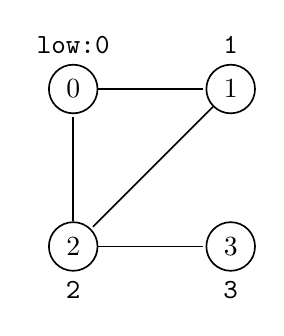
\begin{tikzpicture}[-,>=stealth',shorten >=1pt,auto,node distance=2cm,
                    semithick]
    \tikzset{every state/.style={minimum size=0pt}}
    \node[state,label=above:\texttt{low:0}] (0) {0};
    \node[state,label=above:\texttt{1}] (1) [right of=0] {1};
    \node[state,label=below:\texttt{2}] (2) [below of=0] {2};
    \node[state,label=below:\texttt{3}] (3) [right of=2] {3};
    \path
    (0) edge node{} (1)
    (1) edge node{} (2)
    (2) edge node{} (3)
    (2) edge node{} (0);
\end{tikzpicture}

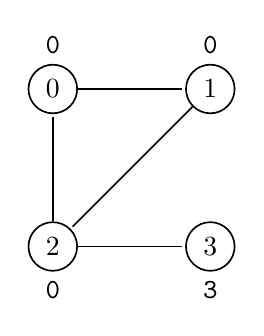
\begin{tikzpicture}[-,>=stealth',shorten >=1pt,auto,node distance=2cm,
                    semithick]
    \tikzset{every state/.style={minimum size=0pt}}
    \node[state,label=above:\texttt{0}] (0) {0};
    \node[state,label=above:\texttt{0}] (1) [right of=0] {1};
    \node[state,label=below:\texttt{0}] (2) [below of=0] {2};
    \node[state,label=below:\texttt{3}] (3) [right of=2] {3};
    \path
    (0) edge node{} (1)
    (1) edge node{} (2)
    (2) edge node{} (3)
    (2) edge node{} (0);
\end{tikzpicture}
\end{multicols}

You can see that \texttt{ids[2] < low[3]}.

\clearpage % Gives us a page break before the next section. Optional.
\section*{Sample}
id: \quad tags: \\
Par
\begin{tabular}{ll}
    \texttt{i}  & par1 \\
    \texttt{j}  & par2 \\
    \texttt{k}  & par3 \\
\end{tabular}

Alg
\begin{enumerate}
\item
    todo
\item
    todo
\item
    todo

\end{enumerate}
\
\section*{}



\begin{comment}
\begin{equation*}
\begin{split}
    \mathcal{L}(H(S), \lambda) 
    &= \sum_{i=1}^9 p_i \log_3{\frac{1}{p_i}} + \lambda \left(\sum_{i=1}^9 p_i - 1 \right) \\
    \pdv{\mathcal{L}}{p_i}
    &= -\log_3{p_i} - \frac{1}{\ln{3}} + \lambda = 0 \quad i \in \{1,2,\dots,9\} \\
    \pdv{\mathcal{L}}{\lambda}
    &= \sum_{i=1}^9 p_i - 1 = 0 \\
    \therefore p_i &= \frac{1}{9}
\end{split}
\end{equation*}
\end{comment}


\end{document}
